\documentclass[12pt]{report}

\usepackage{graphicx}
\usepackage{listings}
\usepackage{titlesec}
\usepackage{amsmath}
\usepackage{url}
\usepackage{biblatex}
\usepackage{hyperref}
\usepackage{float}
\usepackage{subcaption}
\usepackage{geometry}
\usepackage{xcolor}

\hypersetup{
    colorlinks=true,
    linkcolor=black,
    filecolor=blue,      
    urlcolor=blue,
    citecolor=blue,
    linkbordercolor={0 0 1}
}

\geometry{
    left=20mm,
    right=20mm,
    top=20mm,
    bottom=20mm,
}

\addbibresource{references.bib}

\titleformat{\chapter}[display]
  {\normalfont\huge\bfseries}{\chaptertitlename\ \thechapter}{20pt}{\Huge}

\renewcommand{\chaptername}{Task}

\usepackage{inconsolata}

\lstset{
    basicstyle=\ttfamily,
    language=Octave,
    frame=lines,
    literate={-}{-}1,
    breaklines=true,
}

\title{ID2090 A6}
\author{Anton Beny M S, ME23B015}
\date{May 2024}
\begin{document}

\maketitle
\newpage

\tableofcontents

\newpage

\chapter{Treasure Hunt II}

\section{Introduction}
In this task, we have to search for "legendary pokemon: Arceus". The pokemon is represented as ascii art, and we have to find it in the given repository, by going through all the commits.

\section{Hunt}

\subsection{Running the script}

\begin{figure}[H]
    \centering
    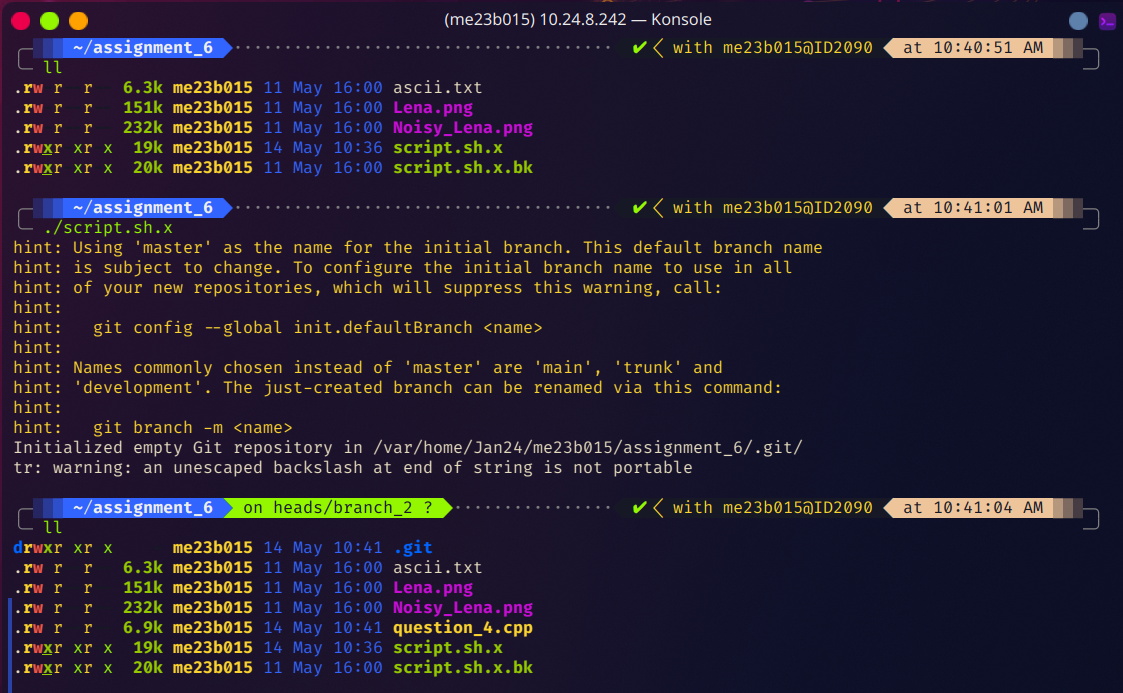
\includegraphics[width=0.8\textwidth]{1_2_0.png}
    \caption{Running the script}
\end{figure}

Upon running the script, we get a git repository with one tracked file "question\_4.cpp".

\subsection{Searching for the pokemon}

\begin{figure}[H]
    \centering
    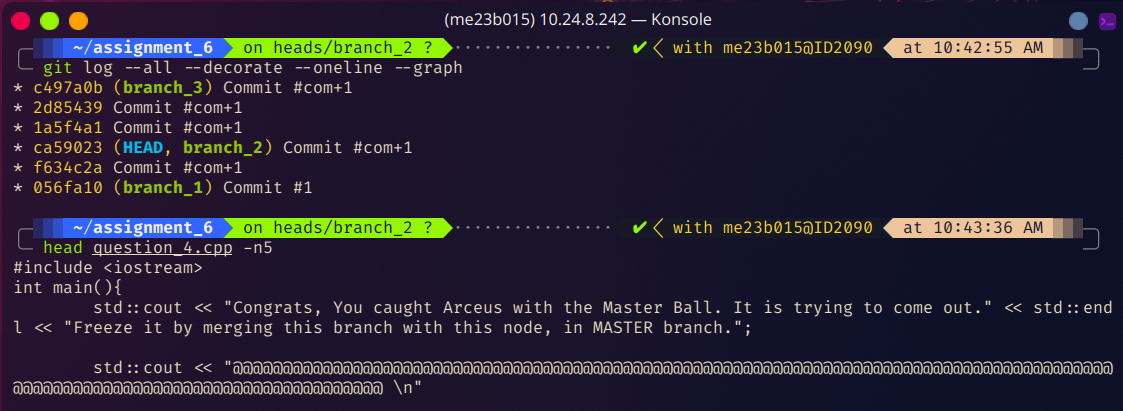
\includegraphics[width=0.8\textwidth]{1_2_1.png}
    \caption{Searching for the pokemon}
\end{figure}

Using \href{https://stackoverflow.com/questions/43549304/how-to-understand-the-graph-output-of-git-log-all-graph-oneline-decorat}{\texttt{git log -all -decorate --oneline --graph}}, we can see that there are a total of 6 commits in the repository. We can use \texttt{git checkout <commit-hash>} in order to go through each commit and find the pokemon.

I found the pokemon in \texttt{branch\_2}.

\subsection{Merging with \texttt{master}}

We need to merge branch\_2 with the \texttt{master} branch. In order to do that, I will first create the \texttt{master} branch using the \texttt{git branch master}. Then, I will checkout to the master using \texttt{git checkout master}.

Finally, I will merge the \texttt{branch\_2} with the \texttt{master} using \texttt{git merge branch\_2}.

\begin{figure}[H]
    \centering
    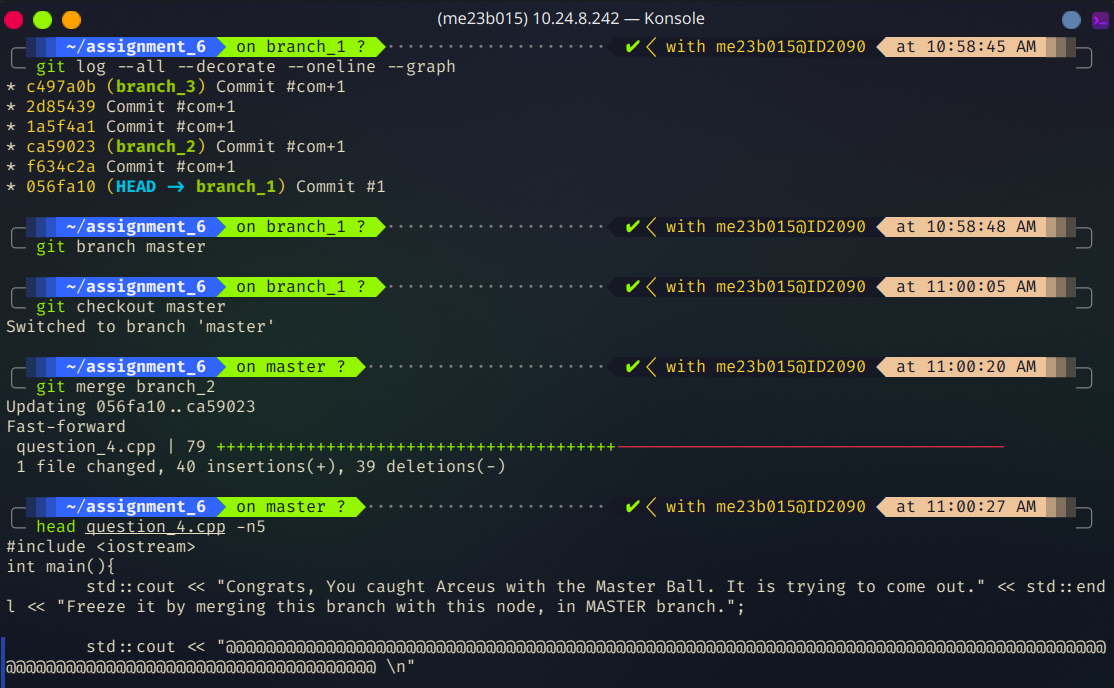
\includegraphics[width=0.8\textwidth]{1_2_2.png}
    \caption{Merging with \texttt{master}}
\end{figure}

\section{Observations}

Here are a few things that I observed, while working on the Task

\begin{itemize}
    \item In my case, after running the script, I was already in \texttt{branch\_2}. Therefore, I didn't need to checkout to other branches.
    \item This was a pretty interesting task. I learnt the basics of git and how to go through the commits in a repository. I also learnt about how to merge branches in git.
\end{itemize}

\newpage

\chapter{Image Processing}

\section{Introduction}

In this task, we have to do some basic image processing, using kernel operations, or in better words, convolutions.

\section{Some Kernels}

\subsection{Brightness Change}

\begin{equation*}
    \begin{bmatrix}
        0 & 0 & 0 \\
        0 & 2 & 0 \\
        0 & 0 & 0
    \end{bmatrix}
\end{equation*}

This kernel will increase the brightness of the image. It is a simple kernel, which will multiply the pixel value by 2, and is capped at 255.

\begin{equation*}
    \begin{bmatrix}
        0 & 0   & 0 \\
        0 & 0.5 & 0 \\
        0 & 0   & 0
    \end{bmatrix}
\end{equation*}

Similarly, we can create a kernel to decrease the brightness of the image.

\begin{figure}[H]
    \centering
    \begin{subfigure}{0.3\textwidth}
        \centering
        \includegraphics[width=\linewidth]{brightened_image.png}
        \caption{Brightened Image}
        \label{fig:f2}
    \end{subfigure}
    \begin{subfigure}{0.3\textwidth}
        \centering
        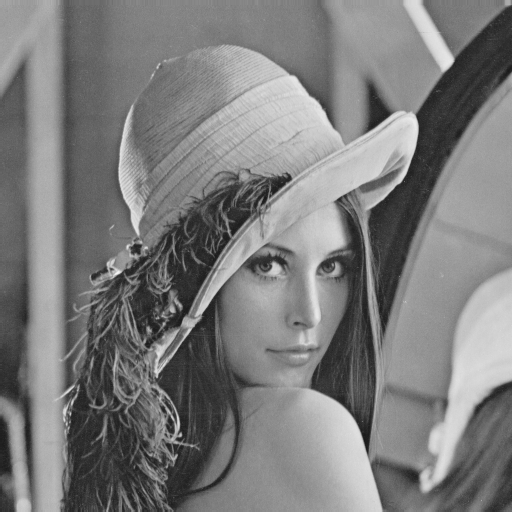
\includegraphics[width=\linewidth]{Lena.png}
        \caption{Original Image}
        \label{fig:f1}
    \end{subfigure}
    \begin{subfigure}{0.3\textwidth}
        \centering
        \includegraphics[width=\linewidth]{darkened_image.png}
        \caption{Darkened Image}
        \label{fig:f3}
    \end{subfigure}
    \caption{Brightness Change}
\end{figure}

\subsection{Edge Detection}

\begin{equation*}
    \begin{bmatrix}
        -1 & -1 & -1 \\
        -1 & 8  & -1 \\
        -1 & -1 & -1
    \end{bmatrix}
\end{equation*}

This kernel works by emphasizing the current pixel value and subtracting the values of the surrounding pixels. This will help in detecting the edges in the image, as the value will be high where there is a sudden change in the pixel values.

\begin{figure}[H]
    \centering
    \begin{subfigure}{0.4\textwidth}
        \centering
        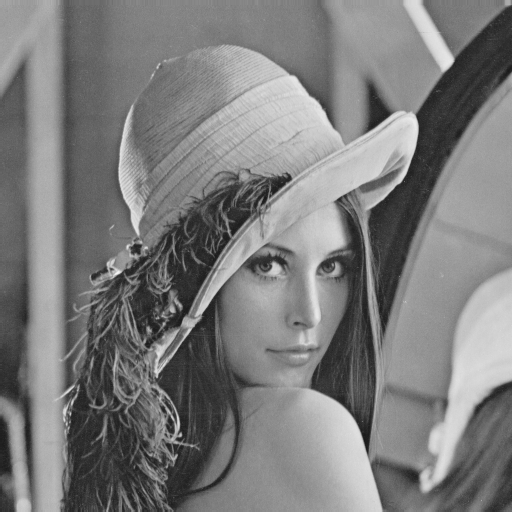
\includegraphics[width=\linewidth]{Lena.png}
        \caption{Original Image}
    \end{subfigure}
    \begin{subfigure}{0.4\textwidth}
        \centering
        \includegraphics[width=\linewidth]{outlined_image.png}
        \caption{Edge Detected Image}
    \end{subfigure}
\end{figure}

\subsection{Blurring}

There are many types of blurring. One of them is box blurring, where the pixel value is the average of the surrounding pixels. This results in smoothening of the image. In this case, equal weights are given to all the surrounding pixels.

\begin{equation*}
    \frac{1}{9} \times
    \begin{bmatrix}
        1 & 1 & 1 \\
        1 & 1 & 1 \\
        1 & 1 & 1
    \end{bmatrix}
\end{equation*}

\begin{figure}[H]
    \centering
    \begin{subfigure}{0.4\textwidth}
        \centering
        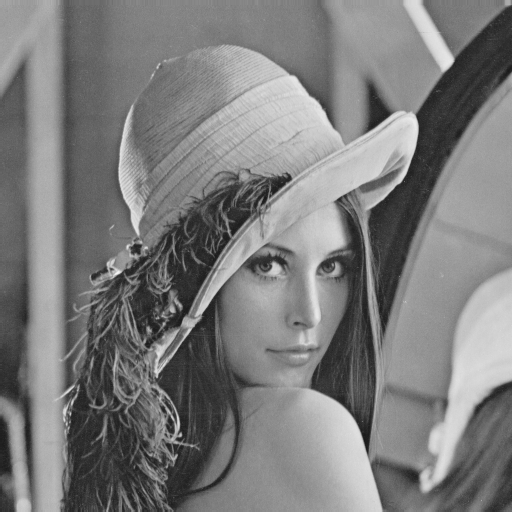
\includegraphics[width=\linewidth]{Lena.png}
        \caption{Original Image}
    \end{subfigure}
    \begin{subfigure}{0.4\textwidth}
        \centering
        \includegraphics[width=\linewidth]{box_blurred_image.png}
        \caption{Box Blurred Image}
    \end{subfigure}
\end{figure}

Another method of blurring is the Gaussian Blur. In this case, the weights are given according to the Gaussian distribution, that is, a higher weight is given to the center pixel, and the weights decrease as we move away from the center. This results in a more natural blur.

\begin{equation*}
    \frac{1}{256} \times
    \begin{bmatrix}
        1 & 4  & 6  & 4  & 1 \\
        4 & 16 & 24 & 16 & 4 \\
        6 & 24 & 36 & 24 & 6 \\
        4 & 16 & 24 & 16 & 4 \\
        1 & 4  & 6  & 4  & 1
    \end{bmatrix}
\end{equation*}

\begin{figure}[H]
    \centering
    \begin{subfigure}{0.4\textwidth}
        \centering
        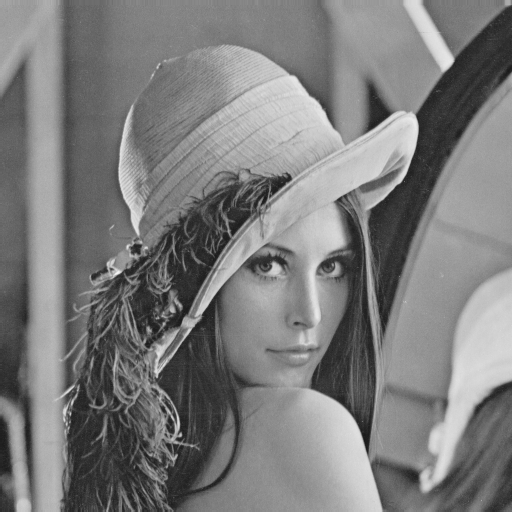
\includegraphics[width=\linewidth]{Lena.png}
        \caption{Original Image}
    \end{subfigure}
    \begin{subfigure}{0.4\textwidth}
        \centering
        \includegraphics[width=\linewidth]{gaussian_blurred_5x5_image.png}
        \caption{Gaussian Blurred Image}
    \end{subfigure}
\end{figure}

\subsection{Sharpening}

Another useful kernel, is the sharpening kernel. This kernel will emphasize the edges in the image, and make the image look sharper.

\begin{equation*}
    \begin{bmatrix}
        0  & -1 & 0  \\
        -1 & 5  & -1 \\
        0  & -1 & 0
    \end{bmatrix}
\end{equation*}

\begin{figure}[H]
    \centering
    \begin{subfigure}{0.4\textwidth}
        \centering
        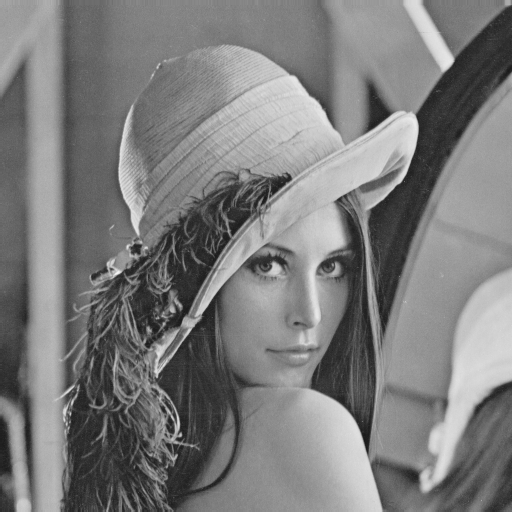
\includegraphics[width=\linewidth]{Lena.png}
        \caption{Original Image}
    \end{subfigure}
    \begin{subfigure}{0.4\textwidth}
        \centering
        \includegraphics[width=\linewidth]{sharpened_image.png}
        \caption{Sharpened Image}
    \end{subfigure}
\end{figure}

\section{Code}

The convolution was done using \texttt{octave}, in a Jupyter environment. The code is as follows:

\subsection{Reading the image}

\begin{lstlisting}[caption={Reading the image}]
image = imread('Lena.png');
imshow(image);
\end{lstlisting}

\subsection{Defining the Kernels}
The following code defines the kernels \cite{enwiki:kernel} that were used in the task.


\begin{lstlisting}[caption={Defining the Kernels}]
brighten = [0, 0, 0; 0, 2, 0; 0, 0, 0];
darken = [0, 0, 0; 0, 0.5, 0; 0, 0, 0];
box_blur = [1, 1, 1; 1, 1, 1; 1, 1, 1] / 9;
gaussian_blur_3x3 = [1, 2, 1; 2, 4, 2; 1, 2, 1] / 16;
gaussian_blur_5x5 = [1, 4, 6, 4, 1; 4, 16, 24, 16, 4; 6, 24, 36, 24, 6; 4, 16, 24, 16, 4; 1, 4, 6, 4, 1] / 256;
unsharp_masking_5x5 = [1, 4, 6, 4, 1; 4, 16, 24, 16, 4; 6, 24, -476, 24, 6; 4, 16, 24, 16, 4; 1, 4, 6, 4, 1] / -256;
sharpen = [0, -1, 0; -1, 5, -1; 0, -1, 0];
outline = [-1, -1, -1; -1, 8, -1; -1, -1, -1];
\end{lstlisting}

\subsection{Defining the Convolution Function}
A function \texttt{convolution} is defined, whose parameters are the image and the kernel. The function returns the convoluted image.

\begin{lstlisting}[caption={The Convolution Function}]
function[output] = convolution(image, kernel)
    [row, col] = size(image);
    [k_row, k_col] = size(kernel);

    delta = (k_row - 1) / 2;
    
    padded_image = zeros(row + 2 * delta, col + 2 * delta);
    padded_image(delta + 1:row + delta, delta + 1:col + delta) = image;

    output = zeros(row, col);

    for i = 1+delta:col+delta
        for j = 1+delta:row+delta
            sub_matrix = padded_image(i-delta:i+delta, j-delta:j+delta);
            output(i-delta, j-delta) = sum(sum(sub_matrix .* kernel));
        end
    end
    output = uint8(output);
end
\end{lstlisting}

\subsection{Generating the images}
Finally, the convolved images are generated using the \texttt{convolution} function, and are saved as images.

\begin{lstlisting}
brightened_image = convolution(image, brighten);
darkened_image = convolution(image, darken);
box_blurred_image = convolution(image, box_blur);
gaussian_blurred_3x3_image = convolution(image, gaussian_blur_3x3);
gaussian_blurred_5x5_image = convolution(image, gaussian_blur_5x5);
unsharp_masking_5x5_image = convolution(image, unsharp_masking_5x5);
sharpened_image = convolution(image, sharpen);
outlined_image = convolution(image, outline);

imwrite(brightened_image, 'brightened_image.png');
imwrite(darkened_image, 'darkened_image.png');
imwrite(box_blurred_image, 'box_blurred_image.png');
imwrite(gaussian_blurred_3x3_image, 'gaussian_blurred_3x3_image.png');
imwrite(gaussian_blurred_5x5_image, 'gaussian_blurred_5x5_image.png');
imwrite(unsharp_masking_5x5_image, 'unsharp_masking_5x5_image.png');
imwrite(sharpened_image, 'sharpened_image.png');
imwrite(outlined_image, 'outlined_image.png');
\end{lstlisting}

\subsection{\href{https://vincmazet.github.io/bip/restoration/denoising.html}{Denoising}}

To remove noise in the given image using kernel operations:

The easiest way to remove noise is to use a \textbf{box blur} kernel. This will average the pixel values and remove some of the noise. However, it also results in loss of detail in the actual image.

\begin{figure}[H]
    \centering
    \begin{subfigure}{0.4\textwidth}
        \centering
        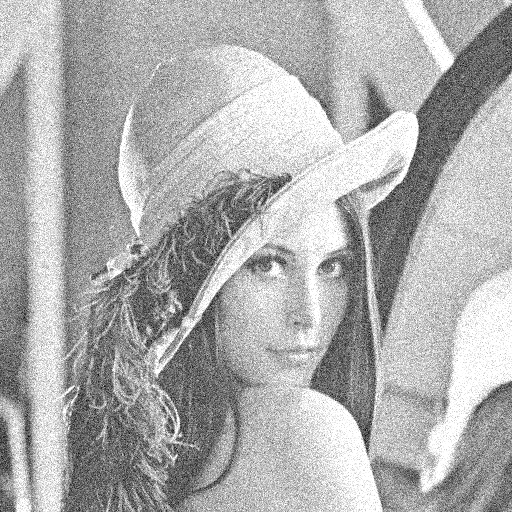
\includegraphics[width=\linewidth]{Noisy_Lena.png}
        \caption{Original Noisy Image}
    \end{subfigure}
    \begin{subfigure}{0.4\textwidth}
        \centering
        \includegraphics[width=\linewidth]{gaussian_blur_denoised_image.png}
        \caption{Denoised Image (Gaussian Blur)}
    \end{subfigure}
\end{figure}

\begin{figure}[H]
    \centering
    \begin{subfigure}{0.3\textwidth}
        \centering
        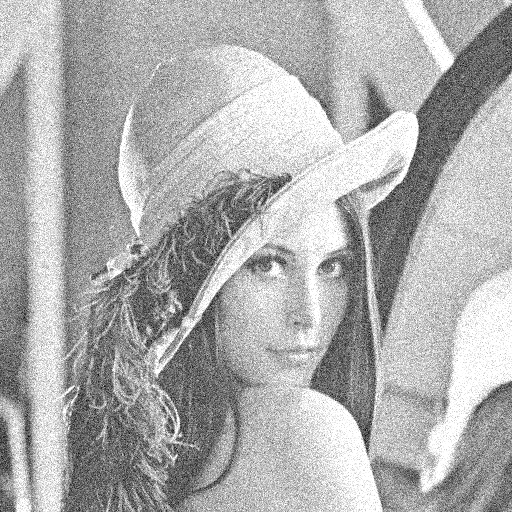
\includegraphics[width=\linewidth]{Noisy_Lena.png}
        \caption{Original Noisy Image}
    \end{subfigure}
    \begin{subfigure}{0.3\textwidth}
        \centering
        \includegraphics[width=\linewidth]{box_blur1_denoised_image.png}
        \caption{Box Blur 1}
    \end{subfigure}
    \begin{subfigure}{0.3\textwidth}
        \centering
        \includegraphics[width=\linewidth]{box_blur2_denoised_image.png}
        \caption{Box Blur 2}
    \end{subfigure}
    \begin{subfigure}{0.3\textwidth}
        \centering
        \includegraphics[width=\linewidth]{box_blur3_denoised_image.png}
        \caption{Box Blur 3}
    \end{subfigure}
    \begin{subfigure}{0.3\textwidth}
        \centering
        \includegraphics[width=\linewidth]{box_blur4_denoised_image.png}
        \caption{Box Blur 4}
    \end{subfigure}
    \caption{Denoising using mutltiple Box Blurs}
\end{figure}

This works becuase, blurring kernels tends to smoothen the image, and in this process, it ends up reducing the noise.

\begin{lstlisting}
t0 = convolution(noised_image, gaussian_blur_5x5);
imwrite(t0, 'gaussian_blur_denoised_image.png');
\end{lstlisting}

\begin{lstlisting}
t0=convolution(noised_image, box_blur);
imwrite(t0, 'box_blur1_denoised_image.png');
t0=convolution(t0, box_blur);
imwrite(t0, 'box_blur2_denoised_image.png');
t0=convolution(t0, box_blur);
imwrite(t0, 'box_blur3_denoised_image.png');
t0=convolution(t0, box_blur);
imwrite(t0, 'box_blur4_denoised_image.png');
\end{lstlisting}

In order to \href{https://mathematica.stackexchange.com/questions/110914/how-to-use-2d-fourier-analysis-to-clean-the-noise-in-an-image}{denoise the image using Fourier Transform}, we can use the following code:

\begin{lstlisting}
[row, col] = size(noised_image);

F = fft2(double(noised_image));
F_shift = fftshift(F);

mask = zeros(row, col);
center = [row/2, col/2];
D0 = 30;
for i = 1:row/2
    for j = 1:col/2
        dist = sqrt((i-center(1))^2 + (j-center(2))^2);
        mask(i, j) = exp(-(dist^2) / (2*(D0^2)));
        mask(row-i+1, j) = mask(i, j);
        mask(i, col-j+1) = mask(i, j);
        mask(row-i+1, col-j+1) = mask(i, j);
    end
end

F_shift = F_shift .* mask;

F = ifftshift(F_shift);

noised_image_denoised = ifft2(F);
noised_image_denoised = real(noised_image_denoised);

imshow((noised_image_denoised));
imwrite(uint8(noised_image_denoised), 'fft_denoised_image.png');
\end{lstlisting}

\begin{figure}[H]
    \centering
    \begin{subfigure}{0.4\textwidth}
        \centering
        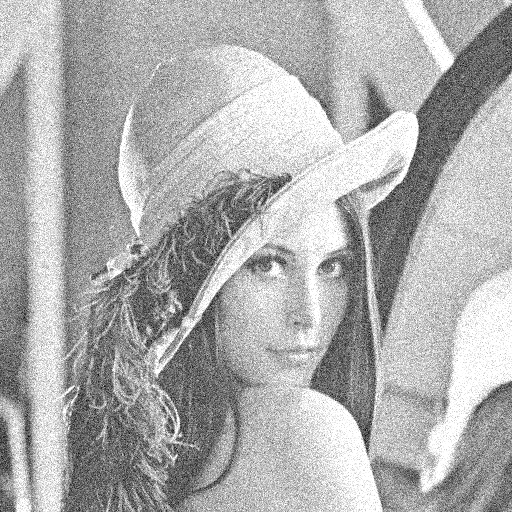
\includegraphics[width=\linewidth]{Noisy_Lena.png}
        \caption{Original Noisy Image}
    \end{subfigure}
    \begin{subfigure}{0.4\textwidth}
        \centering
        \includegraphics[width=\linewidth]{fft_denoised_image.png}
        \caption{Denoised Image (Fourier Transform)}
    \end{subfigure}
\end{figure}

\section{Observations}
\begin{itemize}
    \item Blurring is a simple way to denoise images, but it also results in loss of detail. It is suitable for images where the noise is random and not very large. Threrefore, it is suitable for gaussian noise and salt and pepper noise.
    \item Denoising with Fourier Transform is much \href{https://stackoverflow.com/questions/34027840/removing-periodic-noise-from-an-image-using-the-fourier-transform}{more suitable for images with periodic noise}, as it can be used to remove specific frequencies.
    \item The mask used in the Fourier Transform code is a Gaussian filter, which is used to remove the high frequency noise. For cutoff frequency $D_0 = 30$, the mask is shown here:
          \begin{figure}[H]
              \centering
              \includegraphics[width=0.5\textwidth]{mask_image.png}
              \caption{Mask used in Fourier Transform Denoising}
          \end{figure}
    \item For the boundary pixels, I added the necessary padding, so that the convolved image has the same dimensions as the original image.
\end{itemize}
\section{Conclusion}

\begin{itemize}
    \item I learnt a lot about image processing and how to use kernels to perform operations on images. I also learnt about the Fourier Transform and how it can be used to denoise images.
\end{itemize}

\printbibliography
\end{document}
